\chapter{Wring Components}

\section{Components vs. Service}

\begin{itemize}
  \item \textbf{Component}: reusable piece of software that is used locally,
        eg static/dynamic linking. Is out of control of the writer of the component.
  \item \textbf{Service}: reusable piece of software that is typically accessed
        remotely, either synchronously or asynchronously, eg web service, RPC or soket.
\end{itemize}


\section{Framework}

A framework is a library that provides basic reusable
assets that can be extended by  the developers.
Instead of writing from scatch, use some code that
already exists.

It provides an abstraction layer over lower-level code, allowing developers
to focus on higher-level features.

\begin{tcolorbox}
  \textbf{Note:} Extension and customization are often based on the inversion
  of control.
\end{tcolorbox}

\subsection{Inversion of control}

\begin{quote}
  \centering
  "Don't call us, we'll call you"
\end{quote}


With inversion of control, you code does not control the
overall flow of the program. Instead, a framework or container controls
execution and calls your code at the appropriate time.

\paragraph{Example of direct control}

\begin{center}
  \begin{minipage}{0.65\linewidth}
    \begin{minted}[breaklines]{java}
void main() throws IOException{
  Path path = Path.of("data/grades.csv");
  List<String> lines = Files.readAllLines(path);
  List<String> h = Arrays.asList(lines.get(0).split(","));
  processHeaders(h);
  lines.stream().skip(1)
  .map(r -> Arrays.asList(r.split(",")))
  .forEach(r -> processRow(r));
  
  double average = sum / (lines.size()-1);
  IO.println(average);
}  
\end{minted}
  \end{minipage}%
  \hfill
  \begin{minipage}{0.3\linewidth}
    \centering
    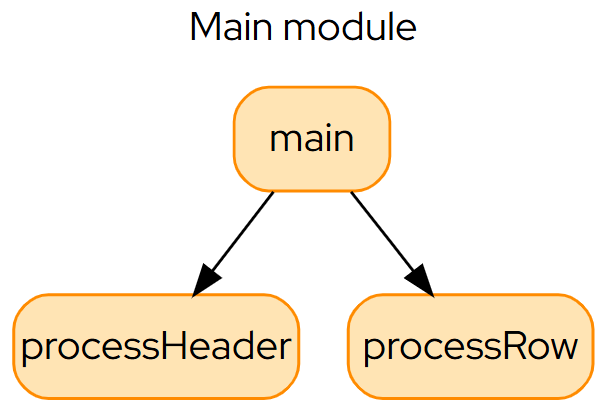
\includegraphics[width=\linewidth]{content/chapters/images/2026-03-27-10-28-11.png}
    \captionof{figure}{Call diagram}
  \end{minipage}
\end{center}


\paragraph{Example of inverted control}

\begin{center}
  \begin{minipage}{0.65\linewidth}
    \begin{minted}[breaklines]{java}
void main() throws IOException{
  CsvReader reader = new CsvReader();
  reader. headerProc(ReadCsvIoC: : processHeaders);

  reader. rowProc(ReadCsvIoC: :processRow);

  int n = reader.read("data/grades.csv");
  IO.println(sum/n);
}
\end{minted}
  \end{minipage}%
  \hfill
  \begin{minipage}{0.3\linewidth}
    \centering
    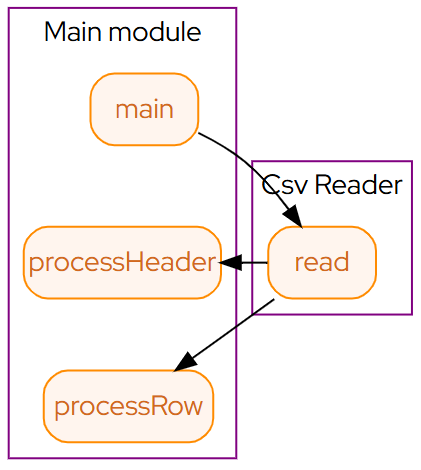
\includegraphics[width=\linewidth]{content/chapters/images/2026-03-27-10-31-01.png}
    \captionof{figure}{Call diagram}
  \end{minipage}
\end{center}


\subsection{Patterns that enable inversion of control}

The \textbf{Template method}, the \textbf{Strategy pattern}, and the \textbf{Observer pattern}
are design patterns that enable inversion of control.


\section{Wiring components}


\subsection{Interacction mode}

\begin{itemize}
  \item \textbf{Call-based}: function or method calls, the base logic of lots
        programming languages.
  \item \textbf{Event-based}: messages are sent and receaved. Used in GUI and
        web applications.
  \item \textbf{state-based}: state is updated and read from a shared memory.
        Used in embedded systems, writing in a specific memory address, and some peripheral devices read  it.
\end{itemize}


\subsection{Call binding}

\begin{itemize}
  \item \textbf{Source inclusion}: The code of the component is included
        directly in the main program during compilation. Strong implementation and compile-time dependecies.
  \item \textbf{Static linking}: Strong implementation dependency,
        limited compile time.
  \item \textbf{Dynamic linking}: Limited implementation dependency,
        limited compile time
  \item \textbf{Dynamic loading}: Strong construction dependency, no
        compile time
\end{itemize}

\subsection{Method/funciton calls}

Problem of simple calls:

\begin{itemize}
  \item Structural dependencies
  \item Runtime dependencies: spacial, temporal and synchronization dependencies
  \item Cascaing failures
  \item Limited scalability
  \item Hard to evolve independently
\end{itemize}

How put toghere components while minimizing the dependencies?
E.g. they are build by different teams with little knowledge of each other.

\paragraph{Example}

A \textit{ThesisLister}, frontend callses, provides a list of thesis matching a
keykords using \textit{ThesisFinder}.

\begin{figure}[h!]
  \centering
  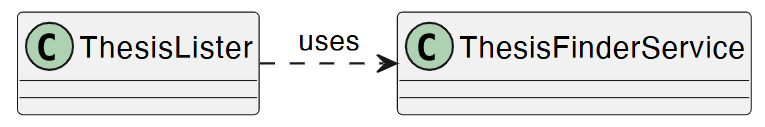
\includegraphics[width=0.3\linewidth]{content/chapters/images/2026-03-27-10-57-22.png}
\end{figure}

Is not testable, not replaceble, heavy dependencies.

Using \textbf{interface} instead of concrete implementation to decouple the components, but still have dependencies.


\begin{figure}[h!]
  \centering
  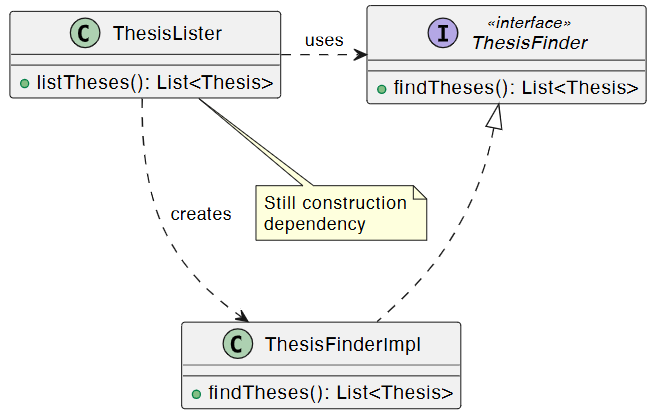
\includegraphics[width=0.3\linewidth]{content/chapters/images/2026-03-27-10-58-21.png}
\end{figure}

\section{Decoupling solutions}

To solve the problem of dependencies, we can use 3 techniques for decoupling components :

\begin{center}
  Dependency injection, Service locator, Message
\end{center}


\subsection{Dependency injection}

The \textit{ThesisLister} calasss id dependent on both the \textit{ThesisFinder} interace and
the implementation of \textit{ThesisFinderImpl}.

The goal of dependency injection is make the lister class unaware of the implementation class,
but can still talk to an instance to do its work.


Move the logic of creating into an \textit{Assembler} class

\begin{figure}[h!]
  \centering
  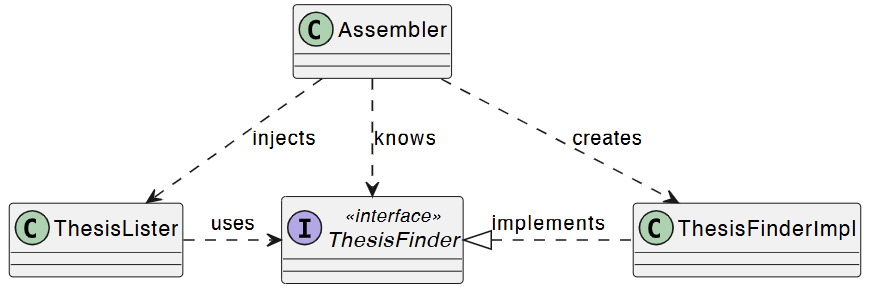
\includegraphics[width=0.3\linewidth]{content/chapters/images/2026-03-27-11-04-05.png}
\end{figure}


How to perfome the injection? Two tecniques:

\begin{itemize}
  \item \textbf{Constructor injection}: use the constructor of the dependent class to inject the dependencies.
  \item \textbf{Setter injection}: objects are initialized with dependency using a
        setter
\end{itemize}


\subsection{Constructor injection}

\begin{figure}[h!]
  \centering
  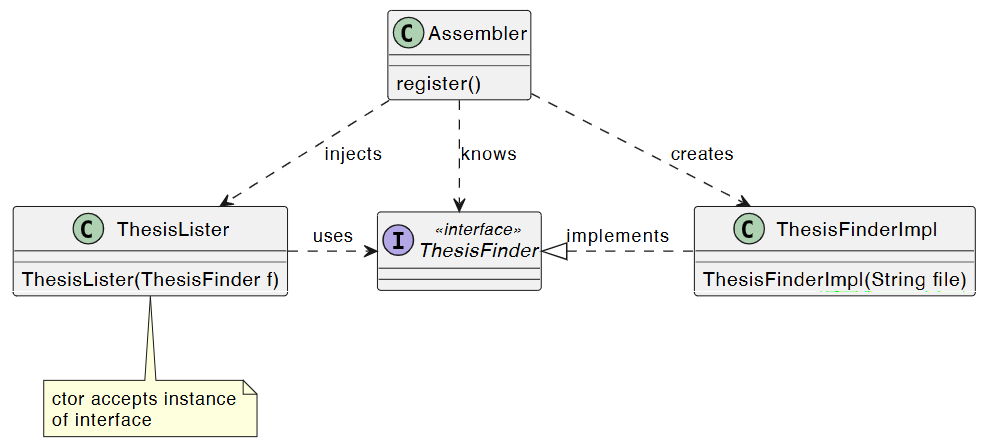
\includegraphics[width=0.3\linewidth]{content/chapters/images/2026-03-27-11-13-04.png}
\end{figure}


\paragraph{Basic injection}

\begin{minted}[breaklines]{java}
ThesisFinder finder = new ThesisFinderImpl(``theses.csv''); //creates the implementation with parameters
ThesisLister lister = new ThesisLister(finder); //injects the dependency upon construction
\end{minted}

\paragraph{Constructor injection with container}

\begin{minted}[breaklines]{java}
Container c = new Container();
Object[] parameters = {"theses.csv"}; //parameters for the implementation ctor
c.registerImplementation(ThesisFinder.class, ThesisFinderImpl.class, parameters); // binding interface to implementation
c.registerComponent(ThesisLister.class); // component registration
\end{minted}

Reflection is used to find out how to link.


\paragraph{Constructor injection with annotations}

\begin{minted}[breaklines]{java}
@Component
public class ThesisFinderImpl implements ThesisFinder {
  public ThesisFinderImpl(@Value("${thesis.file.path}") String file) {
    this. file = file;
  }
}

@Component
public class ThesisLister {
  public ThesisLister(ThesisFinder thesisFinder) {
    this. thesisFinder = thesisFinder;
  }
//...
}
\end{minted}

\begin{tcolorbox}
  \textbf{Note:} The Spring framework is based on constructor injection with annotations.
\end{tcolorbox}


\subsection{Setter injection}

Instead of using the constructor we can use a setter method to inject the dependencies.

\begin{figure}[h!]
  \centering
  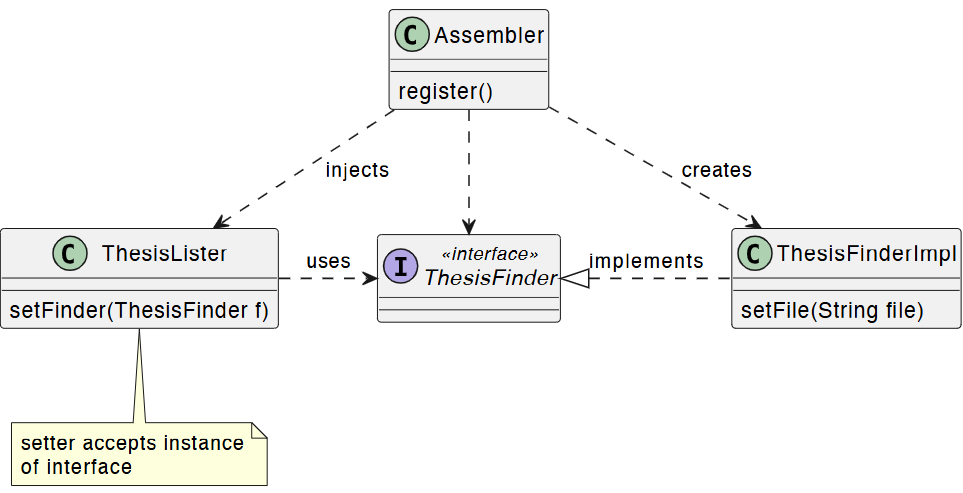
\includegraphics[width=0.3\linewidth]{content/chapters/images/2026-03-27-11-17-52.png}
\end{figure}

\paragraph{Basic injection}

\begin{minted}[breaklines]{java}
ThesisFinderImpl finder = new ThesisFinderImpl(); //creates the server object
finder. setFile("theses.csv");  //set the parameter
ThesisLister lister = new ThesisLister()  //creates the client
lister.setFinder(finder); //injects the dependency with the setter
\end{minted}


To set up a setting injection we can use a confriguation file.


\paragraph{Setter injection with configuration file}

\begin{center}
  \begin{minipage}{0.45\linewidth}
    \begin{minted}[breaklines]{xml}
<beans>
  <bean id="ThesisLister" class="it.polito. ThesisLister">
    <property name="finder">
      <ref local="ThesisFinder"/>
    </property>
  </bean>
  <bean id="ThesisFinder" class="it.polito. ThesisFinder">
    <property name="file">
      <value>theses.csv</value>
    </property>
  </bean>
</beans>
\end{minted}
  \end{minipage}%
  \hfill
  \begin{minipage}{0.45\linewidth}
    \begin{minted}[breaklines]{json}
[
  {
    "id":"ThesisLister",
    "class":"it.polito. ThesisLister",
    "properties": [
      {"name": "finder", "local":"ThesisFinder"}
    ]
  },
  {
    "id":"ThesisFinder",
    "class": "it.polito. ThesisFinderImpl",
    "properties": [
      {"name": "file", "value":"theses.csv"}
    ]
  }
]
\end{minted}
  \end{minipage}
\end{center}



\subsubsection{Setter injection with annotations}

\begin{minted}[breaklines]{java}
@Component
public class ThesisLister {

  private ThesisFinder finder;

  public ThesisLister() {}

  @Autowired
  public void setThesisFinder(ThesisFinder thesisFinder) {
  this. thesisFinder = thesisFinder;
  }
}
\end{minted}



\begin{table}[h!]
  \renewcommand{\arraystretch}{1.4}
  \centering
  \begin{tabularx}{\textwidth}{XXX}
    \hline
    \textbf{Criterion}    & \textbf{Constructor}                              & \textbf{Setter}                                  \\
    \hline
    Mandatory             & Yes (object creation)                             & No (later stage)                                 \\
    Validity              & Yes, always                                       & Only after injection                             \\
    Immutability          & Yes (\texttt{final})                              & No                                               \\
    Null safety           & Fails fast                                        & Risk later \texttt{NullPointerException}         \\
    Understandability     & Depends explicit ctor                             & Depends hidden in setters                        \\
    Circular dependencies & No                                                & Can sometimes resolve                            \\
    Optional dependencies & No, requires \texttt{Optional<>} or ctor overload & Yes (with \texttt{@Autowired(required = false)}) \\
    \hline
  \end{tabularx}
\end{table}


\section{Service locator}


\begin{center}
  \begin{minipage}{0.65\linewidth}
    A service locator is an object that knows how to get hold of all
    of the services that an application might need.

    It is an alternative to dependency injection to break the
    dependencies.

  \end{minipage}%
  \hfill
  \begin{minipage}{0.3\linewidth}
    \centering
    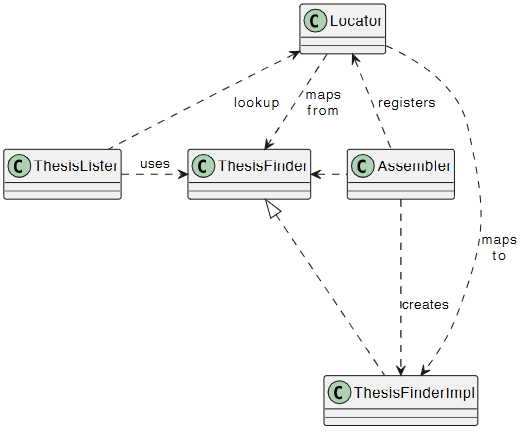
\includegraphics[width=\linewidth]{content/chapters/images/2026-03-27-11-28-56.png}
  \end{minipage}
\end{center}


\paragraph{Example of locator service}
\begin{minted}[breaklines]{java}
public class ThesisLister {
  public static String FINDER_SVC="thesis-finder";
  private final ThesisFinder thesisFinder;

  public ThesisLister() {
    this. thesisFinder = Locator.getLocator().lookup(FINDER_SERVICE, ThesisFinder.class);
  }
//...
}
\end{minted}

\paragraph{Basic assembler}

\begin{minted}[breaklines]{java}
Locator l = Locator.getLocator();
l.register(ThesisLister.FINDER_SVC, new ThesisFinderImpl("theses.csv"));
ThesisLister thesisLister = new ThesisLister();
\end{minted}


\subsection{Locator vs. Dependency injection}


\begin{table}[h!]
  \renewcommand{\arraystretch}{1.4}
  \centering
  \begin{tabularx}{\textwidth}{XXX}
    \hline
    \textbf{Criterion}           & \textbf{Service Locator}              & \textbf{Dependency Injection}           \\
    \hline
    Decoupling                   & Yes                                   & Yes                                     \\
    Mechanism                    & Client explicit lookup                & Provided externally                     \\
    Inversion of Control         & No                                    & Yes                                     \\
    Visibility of dependencies   & Hidden inside method calls to locator & Explicit in constructor/setters         \\
    Dependency on infrastructure & Client depends on the locator         & No dependency on injector/container API \\
    Ease of debugging            & Easier (explicit calls)               & Harder (framework wiring)               \\
    Simplicity                   & Straightforward                       & Less obvious at first                   \\
    Reusability                  & Limited                               & Yes, no assumptions                     \\
    Deferred linking             & Yes, call locator anytime             & No, injected at startup                 \\
    \hline
  \end{tabularx}
\end{table}


\section{Messages/Events}

Replace Direct call with a Broker

\begin{figure}[h!]
  \centering
  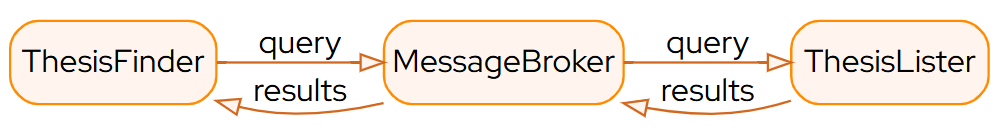
\includegraphics[width=0.3\linewidth]{content/chapters/images/2026-03-27-11-34-23.png}
\end{figure}

In this case sender does NOT know:

\begin{itemize}
  \item Who consumes the message
  \item When the message is processed
  \item How many consumers exist
\end{itemize}

\subsection{Roles: Producer, Consumer}

\begin{table}[h!]
  \renewcommand{\arraystretch}{1.4}
  \centering
  \begin{tabularx}{\textwidth}{X X}
    \hline
    \textbf{Producer}            & \textbf{Consumer}       \\
    \hline
    Sends messages               & Receives messages       \\
    Does not wait for processing & Processes independently \\
    Does not know consumers      & Can scale horizontally  \\
    \hline
  \end{tabularx}
\end{table}


\subsection{Roles: Broker}

The broker, like in real life, is an intermediary that facilitates the communication between producers and consumers.
It's a middleware responsible for:

\begin{itemize}
  \item Storing messages
  \item Delivering messages to consumers
  \item Handling routing and filtering of messages
\end{itemize}

Some examples of brokers areRabbitMQ, ActiveMQ, Kafka, Amazon SQS.



\subsection{Delivery Guarantees}
It is possible to configure different levels of delivery guarantees depending on the requirements of the application.

\begin{table}[h!]
  \renewcommand{\arraystretch}{1.4}
  \centering
  \begin{tabularx}{\textwidth}{X X}
    \hline
    \textbf{Type} & \textbf{Meaning}                             \\
    \hline
    At most once  & messages may be lost                         \\
    At least once & messages may be duplicated, need idempotency \\
    Exactly once  & delivery guarantees, expensive               \\
    \hline
  \end{tabularx}
\end{table}


Distributed systems always involve trade-offs.


\paragraph{Producer Example}
\begin{minted}[breaklines]{java}
ConnectionFactory factory = new ConnectionFactory();
factory.setHost("localhost");

try (Connection connection = factory. newConnection();
Channel channel = connection. createChannel() ) {

  channel.queueDeclare("orders", false, false, false, null);

  String message = "New Order: 123";

  channel.basicPublish("", "orders", null, message.getBytes());
  System.out.println("Sent: " + message);
}
\end{minted}

\paragraph{Producer Example}
\begin{minted}[breaklines]{java}
ConnectionFactory factory = new ConnectionFactory();
factory.setHost("localhost");

Connection connection = factory.newConnection();
Channel channel = connection. createChannel();

channel.queueDeclare("orders", false, false, false, null);

DeliverCallback callback = (tag, delivery) -> {
  String message = new String(delivery.getBody());
  System.out.println("Received: " + message);
};

channel.basicConsume("orders", true, callback, tag -> {});
\end{minted}


\subsection{Structure}

Producer and consumer are independent processes, they can run on different machines and the broker is infrastructure.

\subsection{Shared state example}

\begin{table}[h!]
  \renewcommand{\arraystretch}{1.4}
  \centering
  \begin{tabularx}{\textwidth}{X X}
    \hline
    \textbf{Queue}             & \textbf{Topic}                 \\
    \hline
    1 message $\to$ 1 consumer & 1 message $\to$ many consumers \\
    Work distribution          & Event broadcast                \\
    Load balancing             & Publish/subscribe              \\
    \hline
  \end{tabularx}
\end{table}


\subsection{Effects}


\begin{itemize}
  \item \textbf{Construction decoupling}: producer does not create consumer
  \item \textbf{Spatial decoupling}: producer does not know location of consumer
  \item \textbf{Temporal decoupling}: consumer does not have to be active with producer. Producer does not have to
        block waiting for an answer
  \item \textbf{Data dependency}: data format and schema must be shared
\end{itemize}

\subsection{Challenges}

\begin{itemize}
  \item Difficult debugging
  \item Eventual consistency
  \item Duplicate handling (idempotency!)
  \item Ordering issues
  \item Schema evolution
\end{itemize}



\section{Shared state}
Is a database just storage, or is it a communication mechanism?

Communication via mutations of shared, persistent state. The components
communicate by reading and writing a common data store, no explicit message passing.

\paragraph{Shared state examples}

\begin{itemize}
  \item In-memory global variables
  \item Shared files
  \item Shared database
  \item Distributed cache (Redis)
\end{itemize}

\subsubsection{Communication patterns}

\begin{itemize}
  \item State-based signaling
  \item Polling
  \item Work queue
  \item Derived state sharing
\end{itemize}

\subsection{Effects}
\begin{itemize}
  \item No structural dependencies
  \item Low temporal dependencies: DB is like message broker
  \item Very high data dependency
  \item Simple mental model
  \item Easy querying and debugging
\end{itemize}

\begin{table}[h!]
  \renewcommand{\arraystretch}{1.4}
  \centering
  \begin{tabularx}{\textwidth}{XXX}
    \hline
    \textbf{Aspect} & \textbf{Shared DB}          & \textbf{In-memory Cache (Redis)} \\
    \hline
    Nature          & Persistent system of record & Ephemeral shared memory          \\
    Latency         & Higher                      & Very low                         \\
    Consistency     & Strong                      & Config-dependent                 \\
    Visibility      & High (queryable history)    & Low (state disappears)           \\
    \hline
  \end{tabularx}
\end{table}


% \section{Communication}


% \begin{enumerate}
%   \item The network is reliable
%   \item Latency is zero
%   \item Bandwidth is infinite
%   \item The network is secure
%   \item Topology does not change
%   \item There is only one administrator
%   \item Transport cost is zero
%   \item The network is homogeneous
% \end{enumerate}


% \subsection{}






